% RESULTADOS-------------------------------------------------------------------

\chapter{RESULTADOS E DISCUSSÕES}
\label{chap:resultados}

Utilizando o método de representação de cenários de teste utilizando diagramas baseados em mapas mentais foram criados diagramas para representar cada um dos cenários de teste automatizados para as funcionalidades \textbf{Efetuar Login} (\autoref{fig:testing-mind-map-efetuar-login}), \textbf{Cadastro de Orçamentos} (\autoref{fig:testing-mind-map-orcamentos-cadastro}), \textbf{Listagem e Deleção de Orçamentos} (\autoref{fig:testing-mind-map-orcamentos-listagem-e-delecao}) e \textbf{Edição de Orçamentos} (\autoref{fig:testing-mind-map-orcamentos-edicao}).

            \begin{figure}[!htb]
                \centering
	            \sbox0{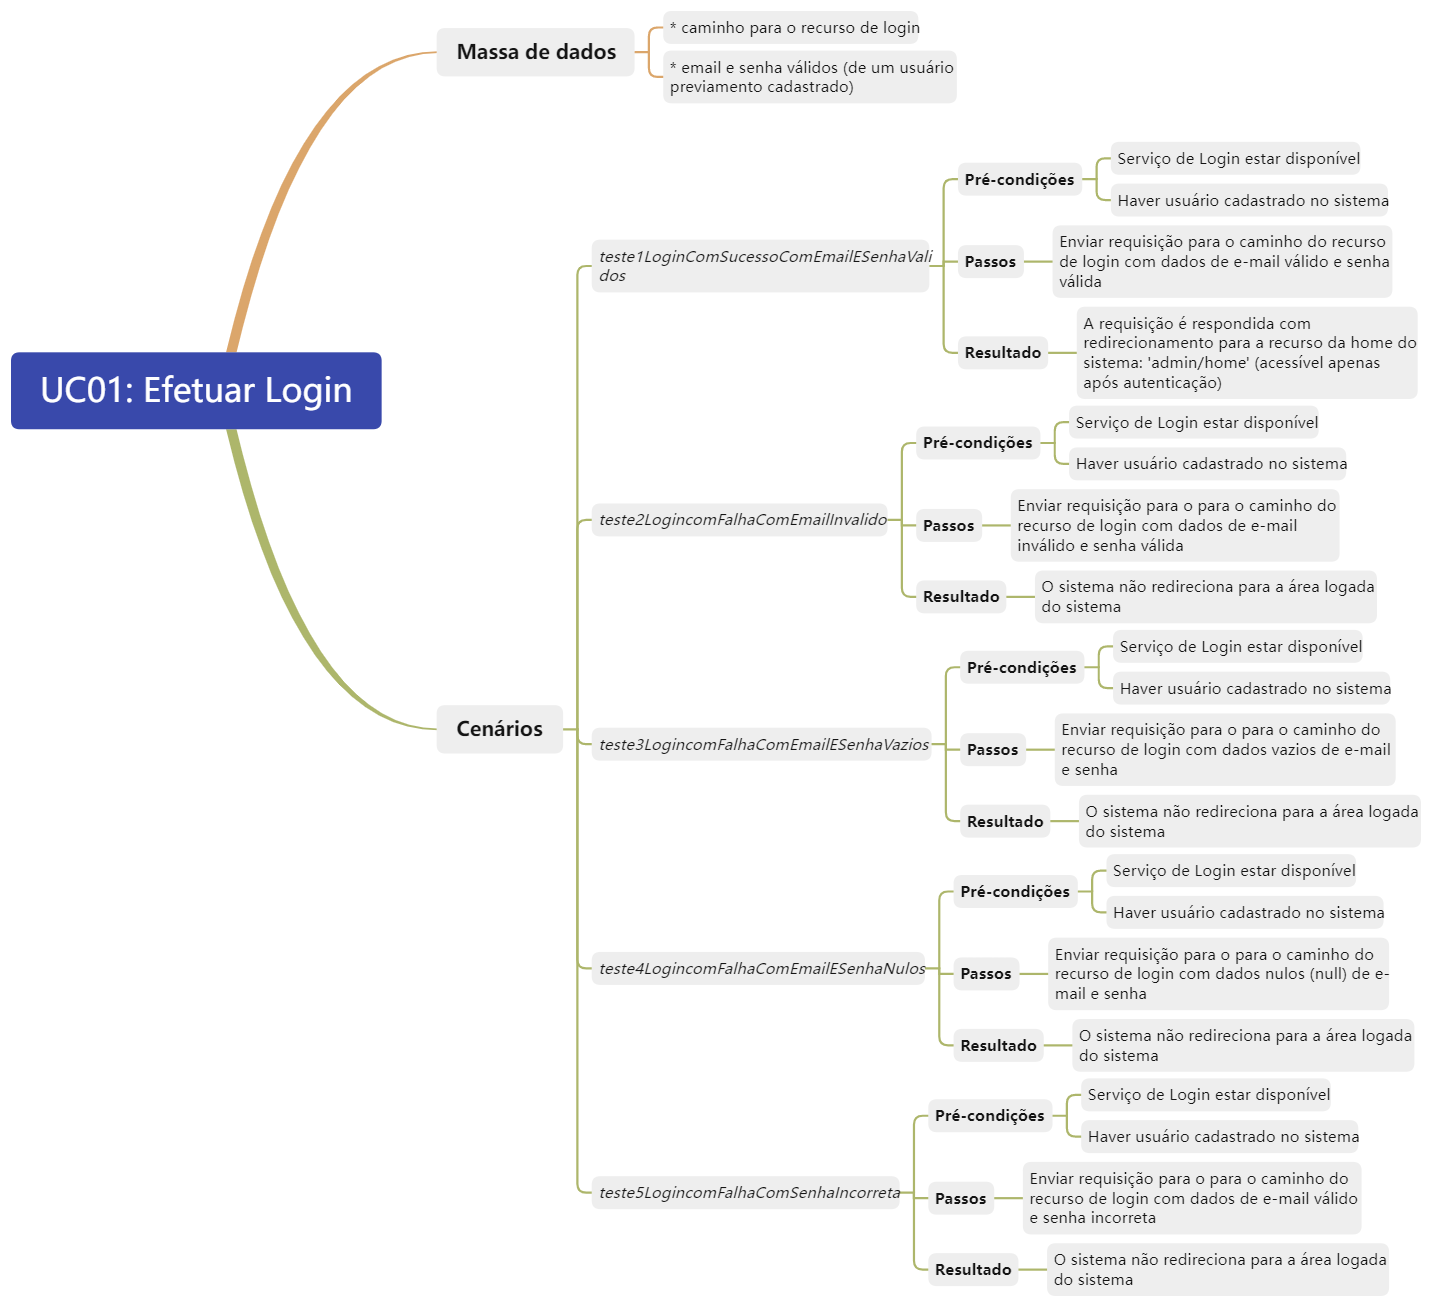
\includegraphics[width=1\textwidth]{./assets/figuras/testing-mind-map-efetuar-login}}% measure width
	            \begin{minipage}{\wd0}
		            \usebox0
		            \caption{Diagrama representando os cenários de teste da funcionalidade \textbf{Efetuar Login}} % Implementação dos cenários de teste de login, baseado na documentação do software e 
		            \label{fig:testing-mind-map-efetuar-login}
		            \fonte{o Autor}
	            \end{minipage}
            \end{figure}

            \begin{figure}[!htb]
                \centering
	            \sbox0{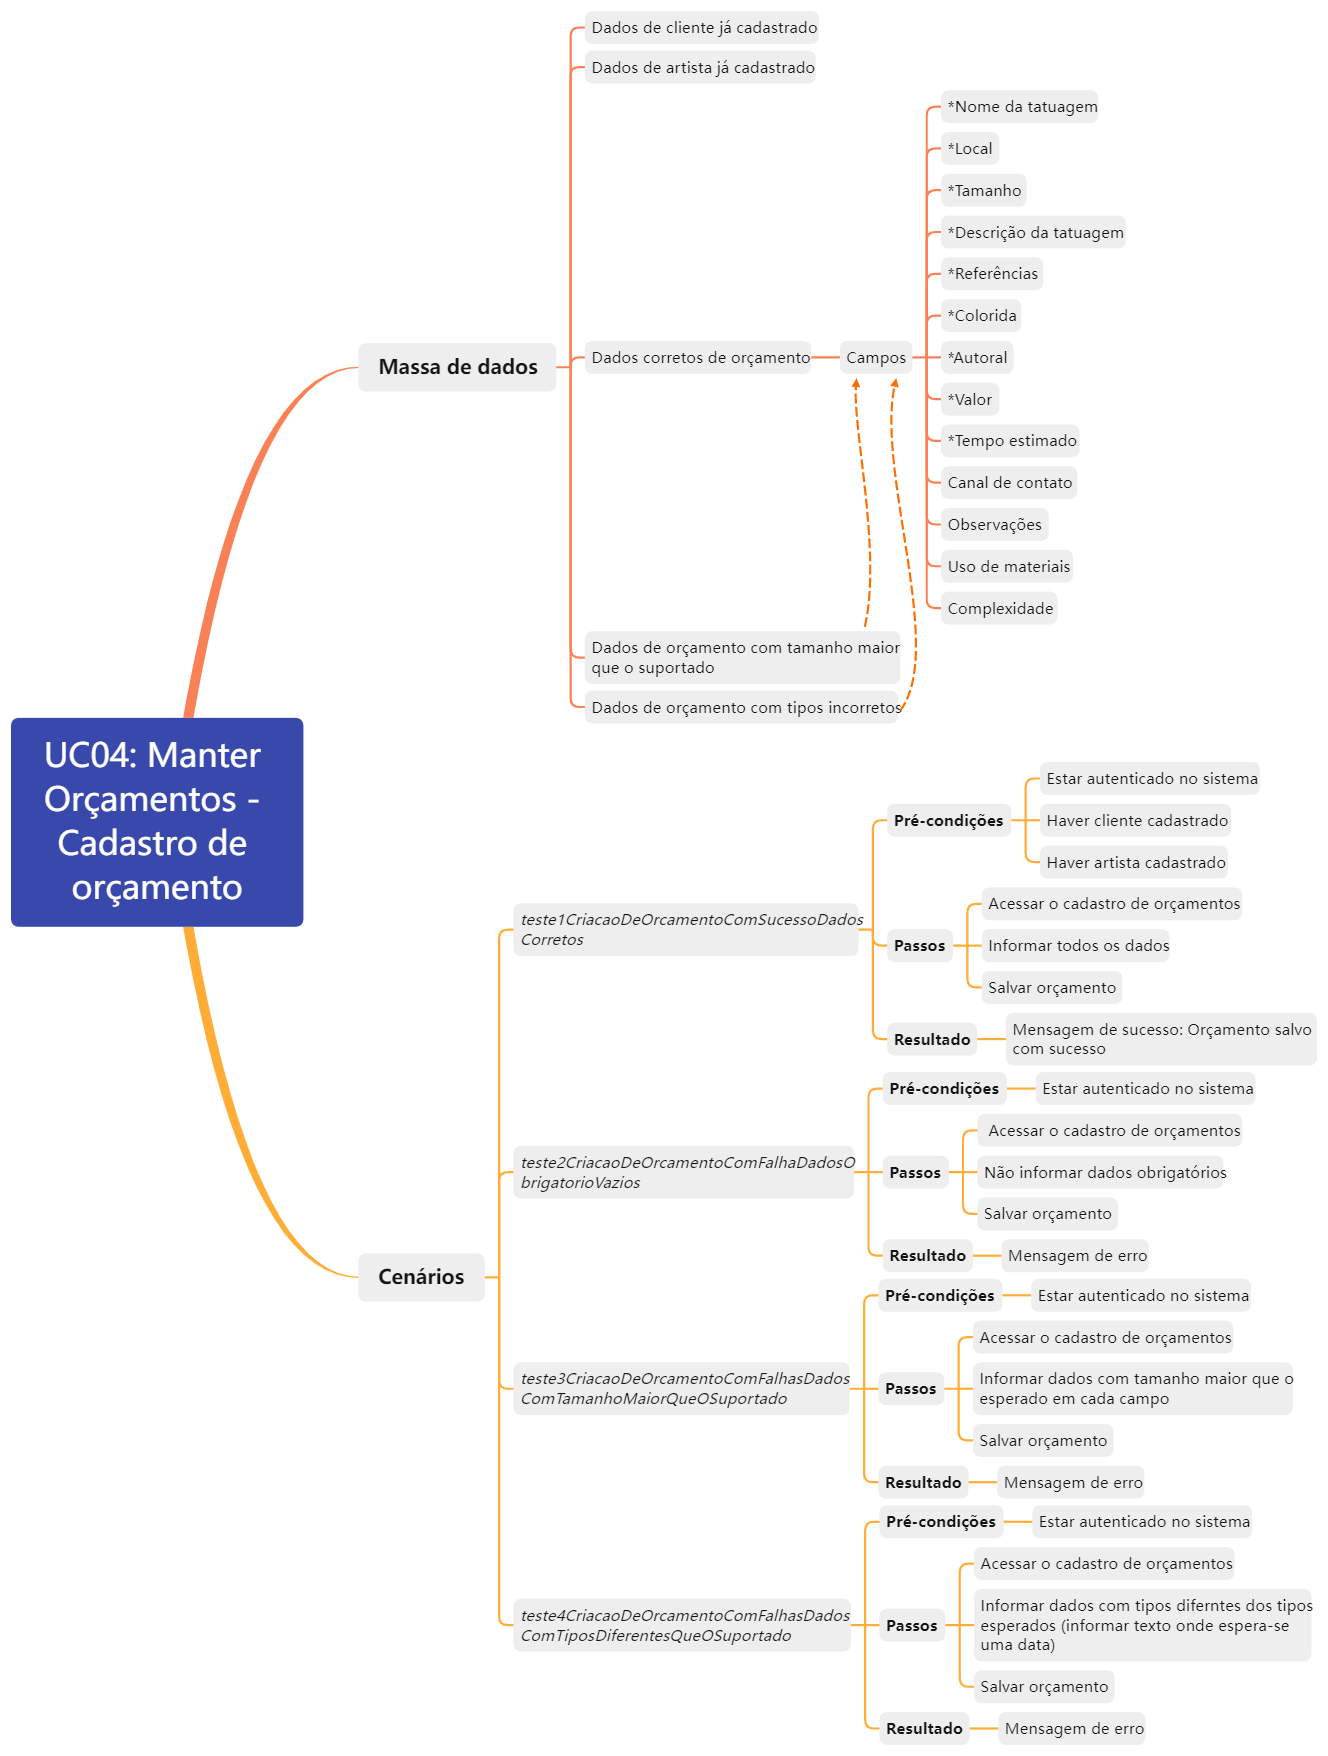
\includegraphics[width=1\textwidth]{./assets/figuras/testing-mind-map-orcamentos-cadastro}}% measure width
	            \begin{minipage}{\wd0}
		            \usebox0
		            \caption{Diagrama representando os cenários de teste da funcionalidade \textbf{Cadastro de Orçamentos}}
		            \label{fig:testing-mind-map-orcamentos-cadastro}
		            \fonte{o Autor}
	            \end{minipage}
            \end{figure}

            \begin{figure}[!htb]
                \centering
	            \sbox0{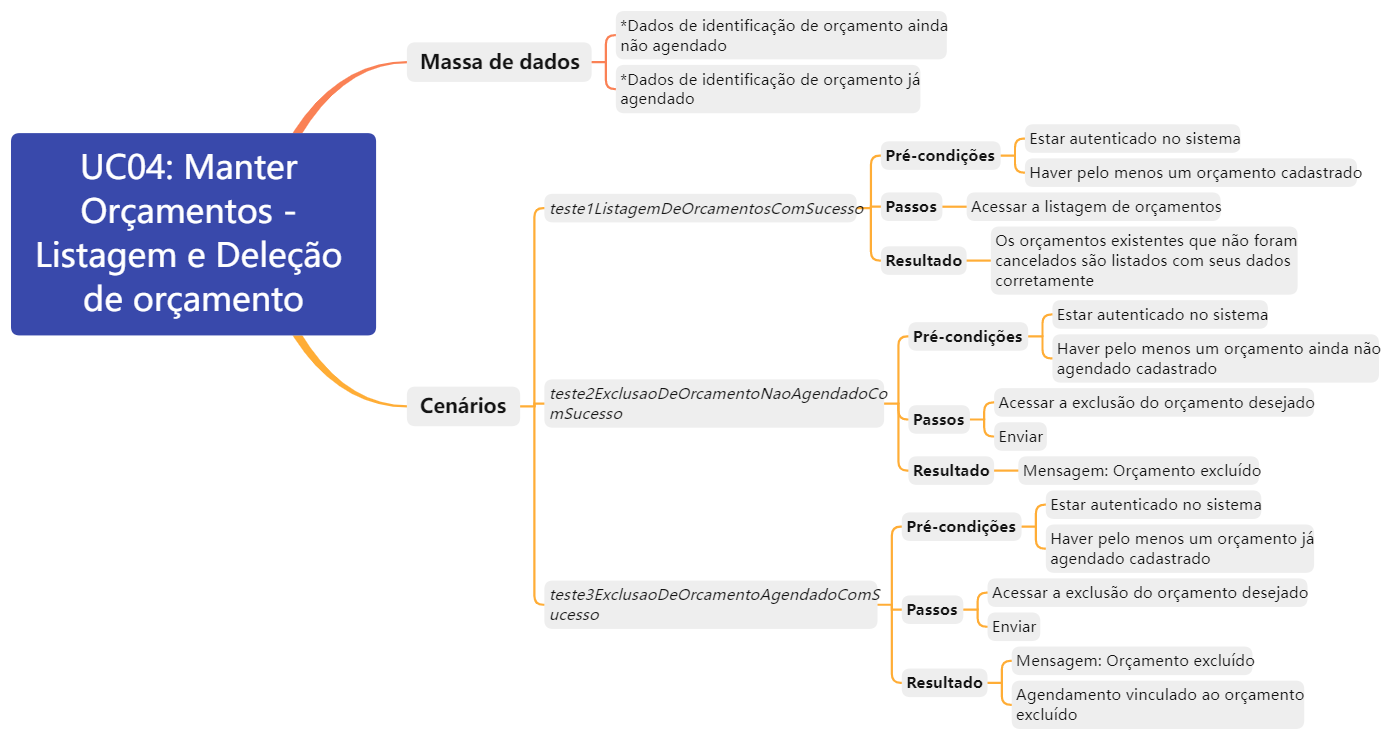
\includegraphics[width=1\textwidth]{./assets/figuras/testing-mind-map-orcamentos-listagem-e-delecao}}% measure width
	            \begin{minipage}{\wd0}
		            \usebox0
		            \caption{Diagrama representando os cenários de teste das funcionalidades \textbf{Listagem e Deleção de Orçamentos}}
		            \label{fig:testing-mind-map-orcamentos-listagem-e-delecao}
		            \fonte{o Autor}
	            \end{minipage}
            \end{figure}

            \begin{figure}[!htb]
                \centering
	            \sbox0{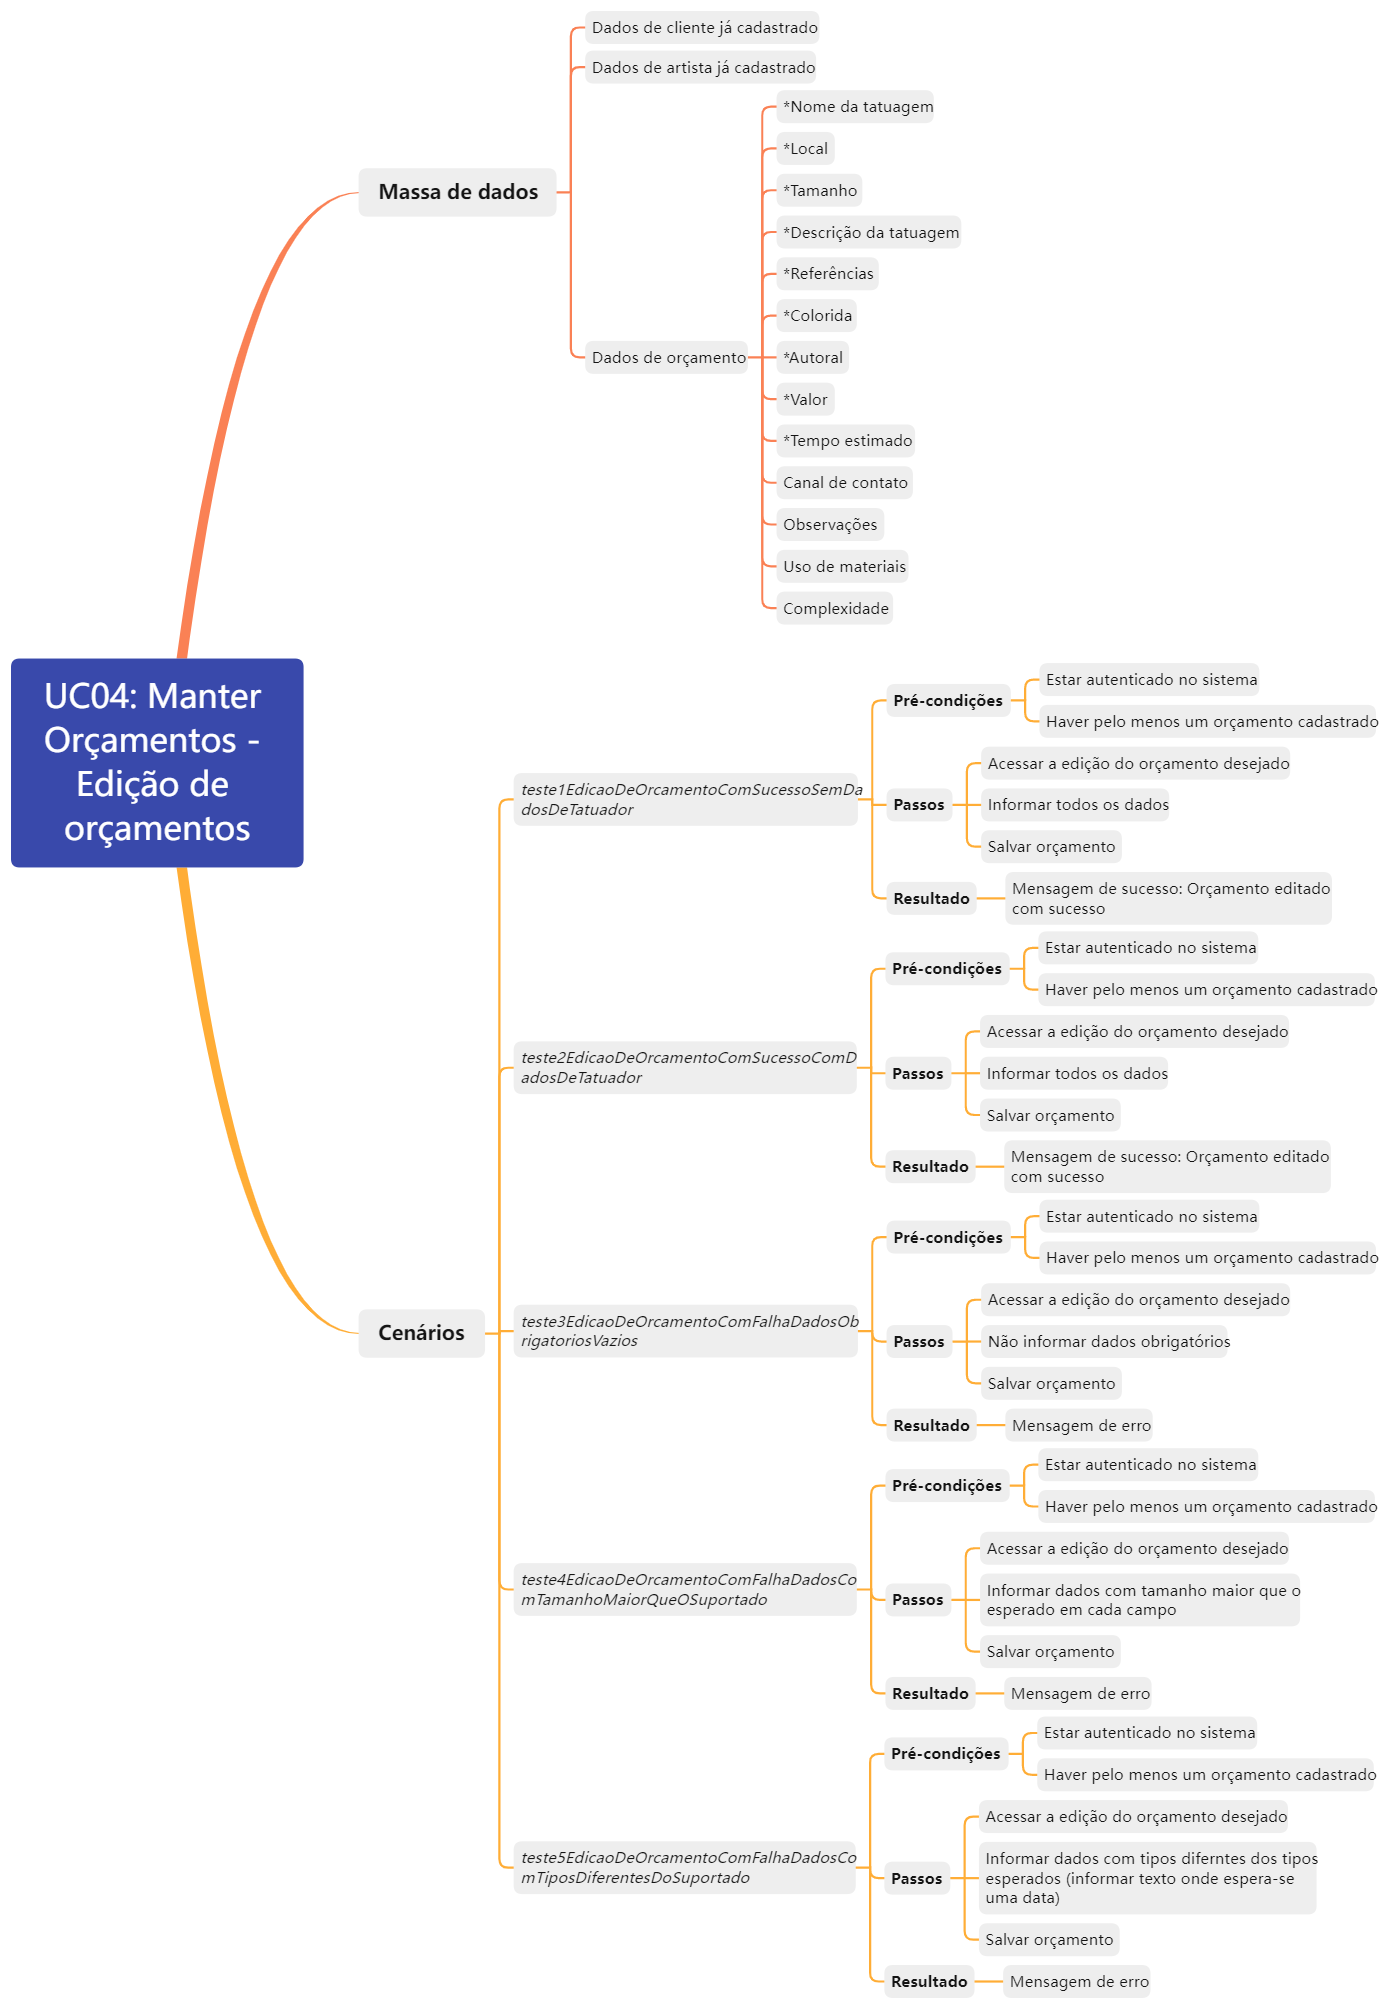
\includegraphics[width=1\textwidth]{./assets/figuras/testing-mind-map-orcamentos-edicao}}% measure width
	            \begin{minipage}{\wd0}
		            \usebox0
            		\caption{Diagrama representando os cenários de teste das funcionalidades \textbf{Edição de Orçamentos}}
		            \label{fig:testing-mind-map-orcamentos-edicao}
		            \fonte{o Autor}
	            \end{minipage}
            \end{figure}

    Em seguida foram criados os \emph{scripts} de teste de integração para os cenários de teste mapeados. O primeiro \emph{script} criado, contém os testes do caso de uso \textbf{Efetuar Login} (\autoref{code:logintest}):
        
    \begin{itemize}
        \item O \emph{script} de teste começa com a declaração da classe de teste e as importações utilizadas nos \emph{scripts} de testes (linhas 1 a 9);
        \item Os métodos de teste são declarados, com o título iniciando sempre pela palavra teste, seguindo a mesma nomenclatura dada aos cenários nos diagramas de planejamento de testes (linha 11);
        \item Abaixo da declaração do método de teste, os objetos e variáveis utilizados no testes são declaradas e instanciadas para serem utilizados nas chamadas (linha 13);
        \item É feita a requisição para o recurso correspondente à funcionalidade testada com os dados de envio necessários, conforme a aplicação foi desenvolvida. A resposta da requisição é armazenada na variável \emph{response} (linha 14);
        \item A asserção verifica o \emph{status code} do retorno da requisição (linha 15) e o redirecionamento para a área do Sistema Admink que é acessível apenas após estar autenticado (linha 16).
    \end{itemize}
        
    %Python code highlighting
\begin{lstlisting}[language=PHP, caption= Cenários de Testes Automatizados de Integração do Login,label={code:logintest}]
<?php

namespace Tests\Integration\Login;

use Tests\TestCase;
use App\User;

class LoginTest extends TestCase
{

    public function teste1LoginComSucessoComEmailESenhaValidos()
    {
        $user = factory(User::class)->create();
        $response = $this->call('POST', '/login', ['email' => $user->email, 'password' => 'teste@123']);
        $response->assertStatus(302);
        $response->assertRedirect('/admin/home');
    }
    
\end{lstlisting}

\fonte{o Autor}
        
    O código realiza a requisição enviando os dados presentes no \emph{script} de teste e por meio das asserções verifica o que foi retornado pelo sistema. Caso o retorno dado pelo sistema seja o esperado na asserção, o teste obtém sucesso, caso contrário o teste falha.
        
    Os objetos instanciados a partir de classes do Sistema Admink foram criados dentro dos \emph{scripts} de teste através das \emph{factories} criadas durante o desenvolvimento do Sistema Admink. As \emph{factories} permitem que os objetos sejam criados com dados aleatórios, possibilitando que diferentes execuções dos testes utilizem diferentes dados, além de permitirem que os comandos para criação dos dados estejam dentro do \emph{script} de teste, removendo a necessidade de que outros \emph{scripts} ou instruções sejam executadas antes dos testes. O uso de \emph{factories} também possibilitou a utilização de um banco de dados \emph{SQLite} específico para os testes. % incluir exemplo no apêndice
        
    Comparando o \emph{script} de teste do cenário  \emph{teste1LoginComSucessoComEmailESenhaValidos} com o diagrama de planejamento de testes é possível visualizar qual parte do \emph{script} cada ramo representa (\autoref{fig:code-and-mind-map}).
        
    \begin{figure}[!htb]
        \centering
	    \sbox0{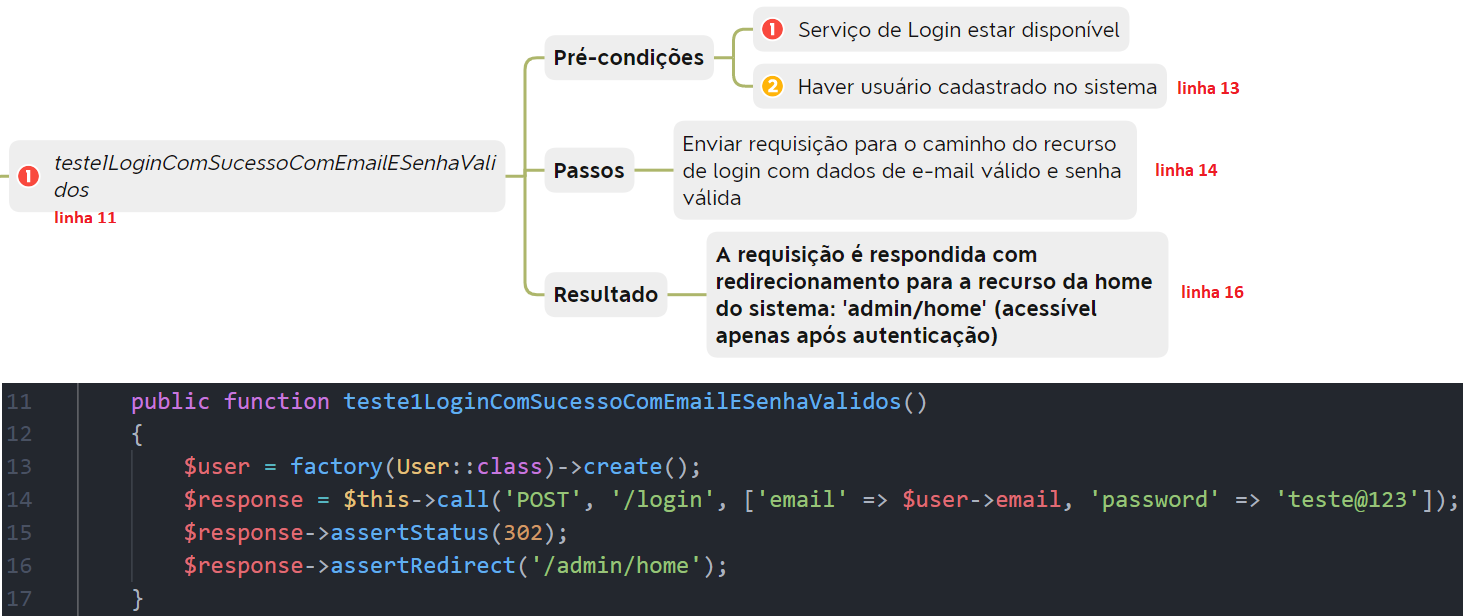
\includegraphics[width=1\textwidth]{./assets/figuras/code-and-mind-map}}% measure width
        \begin{minipage}{\wd0}
	        \usebox0
	        \caption{Comparação do diagrama com o script de teste}
	        \label{fig:code-and-mind-map}
	        \fonte{o Autor}
        \end{minipage}
    \end{figure}
        
    Para cada cenário do caso de uso \textbf{Efetuar Login} deve ser elaborado os \emph{scripts} de teste seguindo uma estrutura semelhante ao primeiro cenário descrito, com as respectivas instâncias de dados e asserções que representam o cenário e sua regra de negócio, pois alterando-se os dados de entrada alteraram-se também o comportamento e os resultados esperados.
        
    Os \emph{scripts} de teste para os cenários de teste identificados para as funcionalidades do caso de uso \textbf{Manter Orçamentos} foram criados seguindo uma estrutura similar à dos testes do caso de uso \textbf{Efetuar Login}. O código completo com todos os \emph{scripts} de teste criados pode ser encontrado no (\autoref{chap:apendiceC}).
    % referenciar apêndices
 
    Utilizando a estrutura definida pelo framework \emph{Laravel}, foi realizada a configuração necessária para a execução dos \emph{scripts} de teste nos arquivos de configuração do \emph{PHPunit} e de variáveis de ambiente.
        
    Em seguida os testes criados foram executados e os resultados analisados.
        
    Todos os \emph{scripts} criados foram armazenados no repositório privado do projeto Admink no \emph{Github}, mas também foi criado um repositório público para armazenar e compartilhar o que foi desenvolvido neste trabalho \footnote{https://github.com/QAkarotto/tcc-software-2022}.
        
    Após os testes criados terem sido executados, analisaram-se os resultados das execuções através dos relatório de execução fornecidos pelo \emph{PHPunit} após o término de cada execução (\autoref{fig:test-result}). Foram realizadas 30 execuções sucessivas, e em todas elas os 19 testes e 84 asserções criadas nos \emph{scripts} de teste obtiveram sucesso em suas execuções, não apresentando falhas. O tempo de execução em todas as execuções não ultrapassou 3 segundos e em média levou cerca de 1,6132 segundos (\autoref{tab:execucaoDosTestes}).
    
    \begin{figure}[!htb]
        \centering
        \sbox0{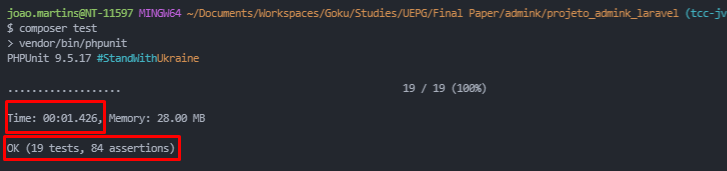
\includegraphics[width=1\textwidth]{./assets/figuras/test-result}}% measure width
        \begin{minipage}{\wd0}
	        \usebox0
	        \caption{Relatório da execução dos testes automatizados destacando em vermelho o tempo de execução e a quantidade de testes e asserções realizadas com sucesso}
	        \label{fig:test-result}
	        \fonte{o Autor}
        \end{minipage}
    \end{figure}
    
    \begin{table}[!htb]
    \vspace{0.5cm}
    \centering
    \begin{tabularx}{\textwidth}{rrrrr}
        \toprule
    & Nº da Execução & Tempo de execução (segundos) \\
        \midrule
             1ª execução	&	1.426	\\
             2ª execução	&	1.312	\\
             3ª execução	&	1.331	\\
             4ª execução	&	1.35	\\
             5ª execução	&	1.383	\\
             6ª execução	&	1.347	\\
             7ª execução	&	1.402	\\
             8ª execução	&	1.365	\\
             9ª execução	&	1.342	\\
            10ª execução &	1.348	\\
            11ª execução &	1.313	\\
            12ª execução &	1.409	\\
            13ª execução &	1.337	\\
            14ª execução &	1.364	\\
            15ª execução &	1.443	\\
            16ª execução &	1.449	\\
            17ª execução &	1.384	\\
            18ª execução &	1.322	\\
            19ª execução &	2.359	\\
            20ª execução &	2.516	\\
            21ª execução &	2.171	\\
            22ª execução &	1.814	\\
            23ª execução &	1.955	\\
            24ª execução &	1.968	\\
            25ª execução &	1.861	\\
            26ª execução &	1.816	\\
            27ª execução &	1.837	\\
            28ª execução &	1.989	\\
            29ª execução &	1.86	\\
            30ª execução &	1.624	\\
        \bottomrule
         Média & 1.613233333
    \end{tabularx}
	\caption[Resultados das execuções scripts de testes]{Resultados das execuções \emph{scripts} de testes.\label{tab:execucaoDosTestes}}
    \fonte{o Autor.}
\end{table}

    
    Foram inseridas alterações nos dados de envio de um dos testes para verificar o que é retornado no relatório de execução em caso de testes falharem. No relatório são exibidas informações indicando quantas falhas foram encontradas, em qual arquivo estão as asserções que falharam, quais asserções falharam e quais foram os valores obtidos comparados aos valores esperados nas asserções, evidenciando o motivo do teste falhar (\autoref{fig:test-fail}).
    
    \begin{figure}[!htb]
        \centering
        \sbox0{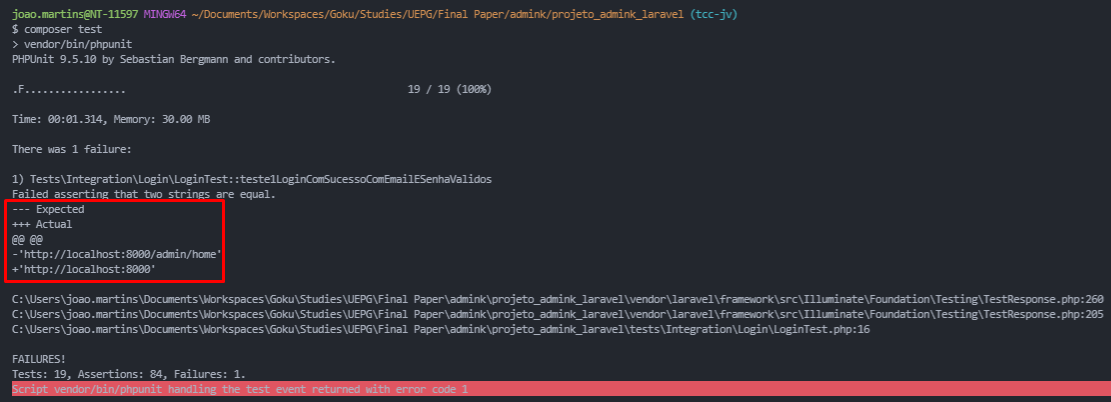
\includegraphics[width=1\textwidth]{./assets/figuras/test-fail-tcc}}% measure width
        \begin{minipage}{\wd0}
	        \usebox0
	        \caption{Exemplo de um teste cuja asserção falhou}
	        \label{fig:test-fail}
	        \fonte{o Autor}
	    \end{minipage}
    \end{figure}
        
    Com os \emph{scripts} criados e suas execuções obtendo sucesso para todos os testes e asserções em poucos segundos, entende-se que a metodologia aplicada na implementação dos testes de integração automatizados foi bem-sucedida e as práticas utilizadas podem ser consideradas para a implementação de testes automatizados de integração. 
    
    Como recomendações propostas por este trabalho, para desempenhar atividades de teste de maneira eficiente deve-se:
    
    \begin{itemize}
        \item Realizar o planejamento dos testes, baseando-se na especificação dos requisitos do software e na aplicação de técnicas de caixa preta, visando identificar os cenários de teste que serão automatizados e quais são os conjuntos de dados que devem ser utilizados nos testes. Caso os \emph{scripts} de teste sejam definidos após a criação do código fonte do software testado, o próprio código fonte somado à aplicação de técnicas de caixa branca pode ser utilizado para auxiliar na identificação dos cenários de teste. Recomenda-se também o uso do método para construção de diagramas de planejamento de testes baseados em mapas mentais como forma de representação dos cenários de teste, evitando a criação de documentos extensos e detalhados;
        \item Consultar a documentação da linguagem de programação ou \emph{framework} utilizado no desenvolvimento do software que será testado, e seguir as recomendações dadas pela documentação a respeito dos \emph{scripts} de teste e configurações necessárias para criação e execução dos mesmos;
        \item Nomear os métodos de teste de acordo com as recomendações da documentação da ferramenta, além de usar a mesma nomenclatura utilizada nos nomes dos cenários de teste identificados. Os nomes devem transmitir claramente o que está sendo verificado pelo método de teste. Desta forma, apesar da nomenclatura dos métodos se tornar verbosa, ela fornece sentido semântico mais rico, e possibilita que os próprios \emph{scritps} de teste sejam parte da documentação do software;
        \item Evitar criar dependências entre diferentes métodos de teste, possibilitando que os métodos possam ser executados em qualquer ordem sem que os testes falhem. Ou seja, os dados e pré-condições necessárias para a execução de um método de teste devem ser providos pelo próprio método, ou então, por um método auxiliar de configuração que é executado antes de todo método de teste ser executado;
        \item Utilizar bancos de dados criados especificamente para os testes, evitando que possua dados que não foram inseridos pelos testes ou como preparação para a execução dos testes. Com o apoio de \emph{migrations} \footnote{permite que o esquema (\emph{schema}) do banco de dados seja definido e possa ser compartilhado,bastando executar a \emph{migration} para atualizar o esquema, além de serem agnósticas de banco de dados, possibilitando a utilização do mesmo código de \emph{migrations} em qualquer sistema gerenciador de banco de dados utilizado} e \emph{factories}, um banco de dados pode ser facilmente criado e populado a cada execução dos testes. Caso não seja possível criar um banco de dados específico para execução dos testes, podem ser utilizados \emph{mock objects}. Entretanto, dessa última forma, não haverá comunicação com um banco de dados real;
        \item Utilizar asserções que obtenham sucesso apenas quando o comportamento esperado realmente foi apresentado pela aplicação. Ou seja, as asserções devem ser precisas e devem evidenciar que o resultado esperado foi obtido.
        \item Armazenar o código criado em um repositório;
    \end{itemize}
    
    As recomendações propostas colaboram para que os \emph{scripts} de teste atendam aos princípios \emph{FISRT} e não possuam \emph{test smells} (\autoref{chap:teste-de-software}) e podem ser inseridas no fluxo de times que utilizam o XP como método ágil, podendo ser realizadas durante a prática do Desenvolvimento Guiado por Testes. Mas também podem ser utilizadas por outros times que também desejem implementar testes automatizados sem ter que criar documentos extensos e detalhados.
    
    Durante a implementação dos testes algumas dificuldades foram encontradas para realizar as asserções devido a forma que a aplicação foi desenvolvida. Nas respostas das requisições realizadas pelos \emph{scripts} de teste sempre é retornado um documento \emph{HTML} como resposta. Dessa forma as asserções devem ser realizadas comparando o conteúdo de campos do \emph{HTML} retornado com os valores esperados. Foi necessário analisar o \emph{HTML} retornado para identificar quais campos continham os dados esperados. Por exemplo no \emph{script} do teste \textbf{teste1ListagemDeOrcamentosComSucesso}  (\autoref{code:teste1ListagemDeOrcamentosComSucesso}):
    
    \begin{itemize}
        \item Nas linhas 18 a 22 é possível visualizar que as asserções estão verificando se o documento \emph{HTML} contem os elementos esperados.
    \end{itemize}
    
    \begin{lstlisting}[language=PHP, caption= Script do teste teste1ListagemDeOrcamentosComSucesso,label={code:teste1ListagemDeOrcamentosComSucesso}]

public function teste1ListagemDeOrcamentosComSucesso()
    {
        $user = factory(User::class)->create();
        $estudio = factory(Estudio::class)->create();
        factory(EstudioUsers::class)->create(['fk_users_id_users' => $user->id, 'fk_estudio_id_estudio' => $estudio->id_estudio]);
        $artista = factory(Artista::class)->create();
        $cliente = factory(Cliente::class)->create();
        factory(ArtistaEstudio::class)->create(['fk_artista_id_artista' => $artista->id_artista, 'fk_estudio_id_estudio' => $estudio->id_estudio]);
        factory(ClienteEstudio::class)->create(['fk_cliente_id_cliente' => $cliente->id_cliente, 'fk_estudio_id_estudio' => $estudio->id_estudio]);
        $orcamento = factory(Orcamento::class)->create(['fk_cliente_id_cliente' => $cliente->id_cliente, 'fk_artista_id_artista' => $artista->id_artista, 'fk_estudio_id_estudio' => $estudio->id_estudio, 'fk_orcamento_status_id_orcamento_status' => 1]);
        $orcamento2 = factory(Orcamento::class)->create(['fk_cliente_id_cliente' => $cliente->id_cliente, 'fk_artista_id_artista' => $artista->id_artista, 'fk_estudio_id_estudio' => $estudio->id_estudio, 'fk_orcamento_status_id_orcamento_status' => 1]);

        $response = $this->actingAs($user)
            ->get('/admin/orcamentos');

        $response->assertStatus(200);
        $response->assertSee('<td class="align-middle">' . $orcamento->tatuagem_nome . '</td>', $escaped = false);
        $response->assertSee('<td class="align-middle">#' . str_pad($orcamento->id_orcamento, 5, '0', STR_PAD_LEFT) . '</td>', $escaped = false);
        $response->assertSee('<td class="align-middle">' . $orcamento2->tatuagem_nome . '</td>', $escaped = false);
        $response->assertSee('<td class="align-middle">#' . str_pad($orcamento2->id_orcamento, 5, '0', STR_PAD_LEFT) . '</td>', $escaped = false);
    }
    
\end{lstlisting}

\fonte{o Autor}
    
    Caso o Sistema Admink tivesse sido desenvolvido para responder as requisições retornando os dados em um documento \emph{JSON} ao invés de diretamente no \emph{HTML} da interface gráfica, a identificação dos campos contendo os dados esperados seria facilitada, assim como a criação das asserções, pois seria necessário verificar apenas os dados do \emph{JSON} e não todo o \emph{HTML}. nas linhas 8 a 10 do \emph{script} de exemplo extraído da documentação do \emph{Framework Laravel} é possível ver como são realizadas asserções para campos de documentos \emph{JSON} (\autoref{code:JSONExampleTest}).
   
    %Python code highlighting
\begin{lstlisting}[language=PHP, caption= Script de Teste exemplificando asserções baseadas em campos de documentos \emph{JSON},label={code:JSONExampleTest}]

public function test_making_an_api_request()
    {
        $response = $this->postJson('/api/user', ['name' => 'Sally']);
 
        $response
            ->assertStatus(201)
            ->assertJson([
                'created' => true,
            ]);
    }
    
\end{lstlisting}

\fonte{o Autor}
    
    Também foram encontradas dificuldades com asserções utilizando os \emph {status codes} retornados nas respostas das requisições. A maioria das requisições realizadas para o Sistema Admink retornam o mesmo \emph{status code} tanto quando se obtém sucesso como quando falha. Para diferenciar sucessos de erros foi necessário analisar as mensagens de sucesso e de erro retornadas nas respostas das requisições, além de utilizar tais mensagens na criação das asserções. Por exemplo nos \emph{scripts} \textbf{teste1CriacaoDeOrcamentoComSucessoDadosCorretos} e \textbf{teste2CriacaoDeOrcamentoComFalhaDadosObrigatorioVazios} (\autoref{code:CriacaoDeOrcamentoTest1E2}):
    
            \begin{itemize}
        \item Na linha 30 é possível ver que a asserção está sendo realizada para o \emph{status code} 302;
        \item Na linha 31 é realizada uma asserção para o texto da mensagem de sucesso na criação de orçamento;
        \item Na linha 58 é realizada asserção também para o \emph{status code} 302, entretanto nesse \emph{script} de teste, obtém-se falha na criação de orçamentos.
        \item Nas linhas 59 a 66 são realizadas asserções para cada uma das mensagens de erros retornadas para cada um dos campos enviados com valores não aceitos. Como o \emph{status code} 302 foi retornado tanto quando se obteve sucesso como quando houve erro na criação de orçamento, essas asserções foram necessárias para diferenciar respostas de sucesso das de erro.
    \end{itemize}
    
    \begin{lstlisting}[language=PHP, caption= Script de testes \textbf{teste1CriacaoDeOrcamentoComSucessoDadosCorretos} e \textbf{teste2CriacaoDeOrcamentoComFalhaDadosObrigatorioVazios}  que testam a criação de orçamentos com sucesso e falha respectivamente, label={code:CriacaoDeOrcamentoTest1E2}]

public function teste1CriacaoDeOrcamentoComSucessoDadosCorretos()
    {
        $user = factory(User::class)->create();
        $estudio = factory(Estudio::class)->create();
        factory(EstudioUsers::class)->create(['fk_users_id_users' => $user->id, 'fk_estudio_id_estudio' => $estudio->id_estudio]);
        $artista = factory(Artista::class)->create();
        $cliente = factory(Cliente::class)->create();
        factory(ArtistaEstudio::class)->create(['fk_artista_id_artista' => $artista->id_artista, 'fk_estudio_id_estudio' => $estudio->id_estudio]);
        factory(ClienteEstudio::class)->create(['fk_cliente_id_cliente' => $cliente->id_cliente, 'fk_estudio_id_estudio' => $estudio->id_estudio]);


        $response = $this->actingAs($user)
            ->post('/admin/orcamentos', [
                'cliente'               => $cliente->id_cliente,
                'artista'               => $artista->id_artista,
                'tatuagem_nome'         => 'Teste Orçamento',
                'tatuagem_local'        => 'Teste',
                'tatuagem_comprimento'  => 10,
                'tatuagem_largura'      => 10,
                'tatuagem_descricao'    => 'Teste Orçamento Criado com Sucesso!',
                'tatuagem_referencias'  => null,
                'canal_contato'         => null,
                'tempo_estimado'        => null,
                'valor'                 => null,
                'uso_materiais'         => null,
                'complexidade'          => null,
                'observacao'            => null
            ]);
        $response->assertStatus(302);
        $response->assertSessionHas('success_toastr', 'O orçamento foi cadastrado com sucesso!');
    }

    public function teste2CriacaoDeOrcamentoComFalhaDadosObrigatorioVazios()
    {
        $user = factory(User::class)->create();
        $estudio = factory(Estudio::class)->create();
        factory(EstudioUsers::class)->create(['fk_users_id_users' => $user->id, 'fk_estudio_id_estudio' => $estudio->id_estudio]);

        $response = $this->actingAs($user)
            ->post('/admin/orcamentos', [
                'cliente'               => null,
                'artista'               => null,
                'tatuagem_nome'         => '',
                'tatuagem_local'        => '',
                'tatuagem_comprimento'  => null,
                'tatuagem_largura'      => null,
                'tatuagem_descricao'    => '',
                'tatuagem_referencias'  => null,
                'canal_contato'         => null,
                'tempo_estimado'        => null,
                'valor'                 => null,
                'uso_materiais'         => null,
                'complexidade'          => null,
                'observacao'            => null
            ]);

        $response->assertStatus(302);
        $this->assertEquals(session('errors')->get('cliente')[0], 'O campo cliente é obrigatório.');
        $this->assertEquals(session('errors')->get('artista')[0], 'O campo artista é obrigatório.');
        $this->assertEquals(session('errors')->get('tatuagem_nome')[0], 'O campo tatuagem nome é obrigatório.');
        $this->assertEquals(session('errors')->get('tatuagem_local')[0], 'O campo tatuagem local é obrigatório.');
        $this->assertEquals(session('errors')->get('tatuagem_comprimento')[0], 'O campo tatuagem comprimento é obrigatório.');
        $this->assertEquals(session('errors')->get('tatuagem_largura')[0], 'O campo tatuagem largura é obrigatório.');
        $this->assertEquals(session('errors')->get('tatuagem_descricao')[0], 'O campo tatuagem descricao é obrigatório.');
    }
    
\end{lstlisting}

\fonte{o Autor}
    
    Caso o Sistema Admink tivesse sido desenvolvido para responder às requisições retornando \emph{status codes} apropriados dependendo do resultado do processamento de cada requisição (por exemplo 201 para sucesso na criação e 400 para dados com valores não aceitos), o \emph{status code} já seria suficiente para diferenciar retornos de sucesso dos de erro, podendo ser usado nas asserções ao invés de apenas o \emph{status code} 302. 